\chapter{Le modeleur open source}

L'intégration d'un plugin Test Designer pour Papyrus a nécessité une phase d'exploration. Celle-ci a permis de mettre en évidence des correspondances entre les librairies RSM et Papyrus. A la suite de cette exploration, un certain nombre de décisions concernant la réorganisation de module en plugin a été planifié.

\subparagraph*{}
L'amélioration du \build a fourni une aide précieuse dans le déploiement d'autres plugins. 
Cela a contribué à la fragmentation en plugins.

\subparagraph*{}
Malgré les ressemblances au modeleur RSM, certaines spécificités ont du être développées pour le modeleur Papyrus.
A la suite de quoi, j'ai étudié le mécanisme de point d'extension d'Eclipse.

\section{Étude du modeleur Papyrus}

Cette partie traite de l'exploration menée sur le modeleur Papyrus.
Elle permet de mettre en évidence les actions à mener, pour créer un plugin exporter pour Papyrus.
Aux vues des premières constatations sur l'ensemble des plugins utilisés par le modeleur.
La ressemblance avec le modeleur RSM fut constatée.

\subparagraph*{}
Papyrus est un modeleur en cours de développement par le CEA\footnote{Commissariat à l'Energie Atomique}.
Il est actuellement livré dans sa version 1.11 mais la version 2 est en cours de développement.
Avec ce modeleur certaines fonctionnalités n'ont tout simplement pas été développées.

Pour étudier le modeleur Papyrus, j'ai téléchargé le code source du modeleur\footnote{Disponible sur https://speedy.supelec.fr/Papyrus/svn/Papyrus/core/releases/1.11.0/}.

\subparagraph{Fonctionnalités non fonctionnelles : }
\begin{itemize}
  \item Impossibilité de réaliser des transitions internes dans un diagramme d'état.
  \item Initialisation automatique des liens entres deux instances d'objet.
  \item Impossible de définir des stéréotypes manuellement.
\end{itemize}

\subparagraph{CEA :}
C'est un acteur majeur en matière de recherche, de développement et d’innovation, le CEA intervient dans trois grands domaines :
\begin{itemize}
  \item  l’énergie
  \item les technologies pour l’information et la santé
  \item la défense et la sécurité
\end{itemize}

\subsection{Points communs}

Les premières constatations du modeleur ont mis en évidence des points communs avec le modeleur RSM.
Papyrus utilise le même framework de stockage du modèle : Emf\footnote{Editing Modeling Framework}.

\subparagraph*{}
Lors de l'exploration, j'ai utilisé le plugin d'exportation d'RSM.
Cela m'a permis de montrer une grande compatibilité avec ce modeleur et la possibilité de réutiliser le code d'extraction d'un modèle RSM dans Papyrus.
Pour réutiliser ce code, j'ai envisagé de fragmenter le plugin ``RSM Exporter'', et créer un autre plugin ``Emf Exporter''.
Cela a pour but de garder uniquement le code spécifique à chaque modeleur dans leur plugin respectif.

\subparagraph*{}
Il n'y a toute fois pas que des points communs.

\subsection{Différences}

\subparagraph{Manque d'utilitaires :}
Comme Papyrus est un modeleur incomplet, il manque d'utilitaires qui permettent de faciliter l'exportation du modèle UML.
Dans RSM, il y a par exemple, une classe qui retourne la liste des modèles ouverts.
Ainsi à partir de celle-ci et du projet en cours de sélection, le modèle du projet sélectionné est récupéré.

\subparagraph*{}
Dans l'interface graphique quelque soit la version d'RSM, il faut ouvrir au moins un élément pour pouvoir accéder au modèle.
Comme on peut le voir sur la figure \ref{OpenProject} p.\pageref{OpenProject}, il y a une différence entre projet ouvert et fermé. 
Tant que le modèle n'a pas été chargé en mémoire, il est impossible d'en extraire les données pour les exporter vers ``Test Designer''. C'est une particularité du modeleur que n'a pas ``Together''.

\begin{figure}[!h]
\begin{center}
  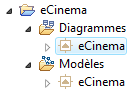
\includegraphics[scale=.7]{images/RsmOpenProject.png}
   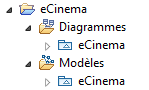
\includegraphics[scale=.7]{images/RsmOpenProject2.png}
  \caption{Projet non ouvert / Projet ouvert}
  \label{OpenProject}
\end{center}
\end{figure}

\subparagraph*{} 
En fait les données du projet RSM sont stockées dans un fichier ``emx''. 
Ce fichier est un document XMI\footnote{XML\footnote{Extensible Markup Language} Metata Interchange} utilisé par le framework Emf pour y stocker les données du modèle. 
Il s'agit d'un framework Java et un générateur de code pour les applications basées sur les modèles structurés. Il permet de prendre en compte toutes les informations contenues dans les diagrammes UML\footnote{Unified Modeling Language}.

\subparagraph{Edition du modèle :}
Quelque soit le modeleur, il existe une fonctionnalité dans l'exporter de modèle qui permet de définir un filtre sur des suites du modèle.
La particularité de cette propriété, est qu'elle est enregistrée dans le modèle UML.
Ainsi dans RSM, on utilise le framework de stockage des éléments UML pour y stocker une propriété supplémentaire sur l'élément suite.

\subparagraph*{} 
Le principe utilisé dans RSM  pour modifier le modèle, ne peut être utilisé de façon identique dans Papyrus. 
Le manque d'utilitaire empêche la réalisation simple du même procédé.
C'est à la suite de la découverte de cette différence que j'ai étudié la procédure d'édition du modèle d'RSM (paragraphe \ref{subsubsection:EditingDomaine} ''Edition du modèle UML d'RSM'' p.\pageref{subsubsection:EditingDomaine} ).

\subparagraph*{}
Parmi les fonctionnalités du plugin d'exportation seul deux fonctionnalités modifient l'état du modèle :
\begin{itemize}
  \item Le filtre sur les suites. 
  		Une suite est un package UML, qui spécifie l'état initial du modèle de génération de tests.
  \item L'éditeur OCL\footnote{\textit{O}bject \textit{C}onstraint \textit{L}anguage}. Il s'agit d'un plugin développé pour RSM qui permet d'éditer plus facilement une garde et un effet sur une transition dans un diagramme d'état. Il offre notamment la complétion\footnote{Complément automatique} et la coloration syntaxique\footnote{Repésentation des mots-clés sous une police différente pour les mettre en évidence}.
\end{itemize}

\subsection{Structure d'un projet Papyrus}

L'étude de la struture du projet Papyrus a aidé à la récupration du modèle.

\subparagraph*{}
Comme on peut l'observer sur la figure \ref{PapyrusProject} p.\pageref{PapyrusProject}, un projet Papyrus est composé de deux fichiers. Le fichier \texttt{.project} appartient à la plateforme Eclipse.
\begin{itemize}
  \item Fichier \texttt{.di2} : Contient les données graphiques des diagrammes de celui-ci. Il s'agit d'un format Xmi comme RSM mais avec un élément \texttt{<di2>} spécifique.
  \item Fichier \texttt{.uml} : Celui-ci contient les données du modèle UML enregistrées au format Emf (XMI).
\end{itemize}

\begin{figure}[!h]
\begin{center}
  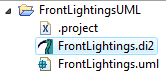
\includegraphics[scale=1]{images/PapyrusProject.png}
  \caption{Fichiers d'un projet Papyrus}
  \label{PapyrusProject}
\end{center}
\end{figure}

\subparagraph*{}
Pour récupérer les données du modèle Emf, il faut utiliser les utilitaires d'Emf pour charger le fichier \texttt{.uml} afin d'en extraire les données UML. C'est à partir de ces données que l'exportation du modèle Emf vers ``Test Designer'' est effectuée.

\subparagraph*{}
A partir de ces données est-il possible de les modifier ?

\subsection{Edition du modèle UML}\label{subsubsection:EditingDomaine}

En l'état, un modèle Emf peut être modifié par des méthodes de modification du modèle.
Hors ce procédé ne peut fonctionner correctement.
Sur un modèle Emf, il est donc obligatoire de passer par un mécanisme centralisé d'édition du modèle.
Ce mécanisme a pour but de modifier le modèle de façon transactionnel.
Toute modification de la propriété d'un élément est réalisée de façon atomique.
Si jamais la modification devait échouée en cours de transaction, le modèle reviendra à l'état précédant.

\subparagraph*{}
Dans Emf, il est appelé ``EditingDomain''.
Les modeleurs sont libres de l'utiliser comme ils le souhaitent.
Il faut de toute façon pouvoir récupérer l'``editingDomain'' des modèles ouverts.
C'est ce que permet de faire RSM via un utilitaire.

\subsection{Récupération d'un modèle}

Papyrus utilise le mécanisme d'adaptation d'Eclipse.
Ce mécanisme permet de retourner un objet instancié par un éditeur ou un objet \texttt{IAdaptable}.
Dans Eclipse, les objets adaptables sont par exemple, les éditeurs et les ressources du projet.

\begin{figure}[!ht]
	\begin{minipage}[c]{0.6\linewidth}
 		\begin{center}
	  		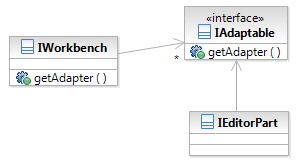
\includegraphics[scale=.6]{images/DiagAdapter.png}
	  		\label{DiagramClassEditor}
	  		\caption{Diagramme de classe d'un éditeur}
		\end{center}
 	\end{minipage}\hfill
 	\begin{minipage}[c]{0.4\linewidth}
 		Tous les éditeurs implémentent \texttt{IEditorPart}. Ainsi tous les éditeurs qui surchargent la méthode  \texttt{getAdapter(Class class)} de l'interface \texttt{IAdaptable} permettent de retourner un objet de la classe passée en paramètre.
 	\end{minipage}
\end{figure}

\subparagraph*{}
C'est ce mécanisme qui a été utilisé dans Papyrus pour récupérer le modèle ouvert.
Exemple, à partir du ``Workbench'' qui est l'espace de travail d'Eclipse. 
Il est possible de demander le modèle UML en faisant : 
\begin{small}
\begin{verbatim}Model theModel = IWorkbench.getAdapter(org.eclipse.uml2.uml.Model.class)\end{verbatim}
\end{small}
Autre exemple si l'on souhaite récupérer un ``editingDomain'', il faudra utiliser :
\begin{small}
\begin{verbatim}EditingDomain editingDomain = IWorkbench.getAdapter(EditingDomain.class)\end{verbatim}
\end{small}
Il y a toute fois un inconvénient à cette solution. Si aucun éditeur n'est ouvert, il n'y a pas de modèle récupérable.

\subsection{Les stéréotypes}

Les stéréotypes sont une fonctionnalité qui a posé problème.
Cette partie a pour but d'expliquer, à quoi ils servent.

\subparagraph*{}
Les stéréotypes sont des propriétés des objets UML, ils permettent de spécifier le comportement de ceux-ci. 
Dans notre cas, d'autres ont été ajoutés pour permettre de spécifier par exemple le comportement d'une opération (figure \ref{stereotype} p.\pageref{stereotype}). 
En spécifiant ``observation'' sur l'opération ``myOperation'' cela signifie que la post condition qui détermine l'état final après exécution de l'opération, ne modifie pas l'état du modèle. 
Et celle-ci doit retourner une valeur. 
Concernant la vérification des stéréotypes, cela est effectué via un contrôle d'erreur au moment de l'exportation du modèle. 
La post-condition est une propriété de l'opération écrit en OCL.

\subparagraph{}
Dans RSM les stéréotypes sont gérés par une extension spécifique au modeleur, qui permet d'ajouter d'autres stéréotypes que ceux standards (interface, abstract, enumeration, \ldots), par exemple : 
\begin{itemize}
  \item observation
  \item setup
  \item teardown
\end{itemize}
Une extension est un mécanisme qui permet d'étendre les fonctions du modeleur à condition que celui-ci l'accepte.

\begin{figure}[!h]
\begin{center}
  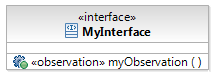
\includegraphics[height=2cm]{images/stereotype.png}
  \caption{Exemple de stéréotype dans RSM}
  \label{stereotype}
\end{center}
\end{figure}

\subparagraph*{}
Quel bilan peut on faire à partir des constations suivantes ?

\subsection{Résultat}

Le bilan de cette étude montre en effet que Papyrus est proche d'RSM.
Toute fois, il est nécessaire que la fragmentation soit effectuée avant de factoriser le code commun pour les deux modeleurs.

Maintenant, concernant les différences et les problèmes constatés en réalité, ceux-ci ne posent aucun problème.
Il y a en effet dans les objectifs de jalon suivant, une modification sur la gestion des suites qui doit supprimer les modifications du modèle. 
Et Smartesting souhaite d'autre part ne plus rien enregistrer dans le modèle.

\subparagraph*{}
Pour l'éditeur OCL, il s'agit d'un plugin qui n'est destiné qu'à RSM.
En sachant que Papyrus n'a pas besoin d'éditer plus facilement une ``garde'' et un ``effet'' car cela l'est suffisamment\footnote{Trois cliques de souris avec Papyrus contre une dizaine avec RSM}.

\subparagraph*{}
Pour la récupération du modèle, il a été fait le choix de récupérer le modèle à partir du fichier \texttt{.uml}.
La manière qui utilise le mécanisme d'adaptation d'Eclipse ne correspond pas à l'attente fonctionnelle du client XP.

\section{Problèmes rencontrés}

Durant l'exploration, un certain nombre de problèmes et de questions ont été soulevés.
Pour certains, il s'agit tout simplement de l'incapacité du modeleur à modéliser pour le test.
Dans d'autres cas, il s'agit d'un fonctionnement qui engendre des erreurs dans le modèle.

Liste des problèmes :
\begin{itemize}
  \item Problème sur les instances de lien dans le modèle
  \item Ajout de nouveaux stéréotypes
  \item Gestion des ranges sur les entiers
  \item Problème d'extraction des commentaires
\end{itemize}

\subsection{Problème sur les instances de lien dans le modèle}

Lorsque l'on souhaite créer un lien entre deux instances dans Papyrus, une erreur non explicite est détectée au moment de l'exportation du modèle.
Après une recherche de la cause possible de cette erreur, nous avons fini par en déduire la cause d'une mauvaise construction du lien dans Papyrus. 
Nous avons constaté que les slots du lien en question, ne sont pas créés automatiquement contrairement à ceux du modeleur RSM.

\subparagraph*{}
La figure \ref{ProblemLink} p.\pageref{ProblemLink} est une capture du modeleur Papyrus qui met en évidence le problème lié à la création de lien d'instance (1).
On peut voir entouré en rouge (2) que les slots ne sont pas initialisés. Pour cela, il faut les initialiser manuellement pour arriver au résultat encadré en orange (3).

\begin{figure}[!ht]
\begin{center}
  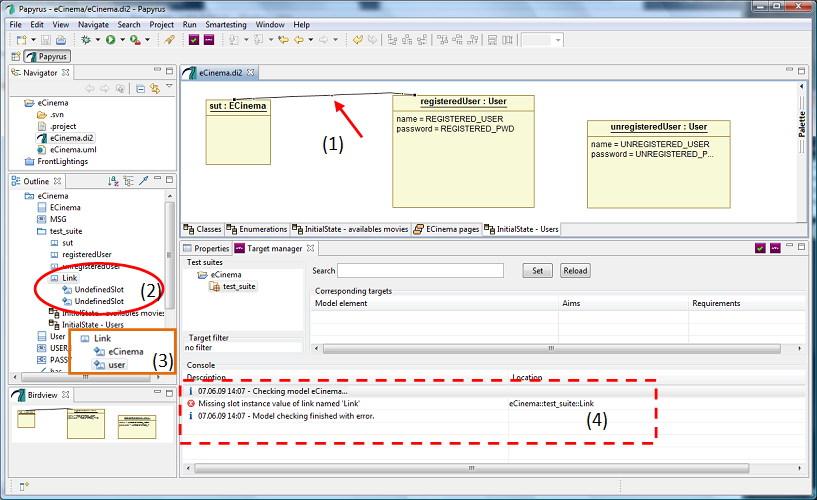
\includegraphics[width=.9\linewidth]{images/Papyrus.png}
  \caption{Modeleur Papyrus - Problème sur le lien entre instances}
  \label{ProblemLink}
\end{center}
\end{figure}

\subparagraph*{}
C'est via ce problème que nous avons mis en évidence un manque de clarté de certains messages d'erreurs pas assez explicites du genre \texttt{NullPointerException} ou \newline \texttt{IndexOutOfBoundException} qui ont été corrigés pour donner le résultat dans l'encadré en pointillés rouges (4) figure \ref{ProblemLink} p.\pageref{ProblemLink}.

\subsection{Gestion des ranges sur les entiers}

La fonctionnalité de range d'entier est réalisée à partir d'un point d'extension spécifique à RSM. Cette fonctionnalité n'existe pas dans le modeleur Together. 
Cette fonctionnalité offre la possibilité de paramétrer graphiquement le range représentant un entier.
Lors de la modélisation pour les tests, les valeurs des paramètres d'entrée d'une opération génèrent autant de cas de tests que de combinaisons de valeurs possibles de ces paramètres. 
Pour diminuer le nombre de tests, on utilise des ranges sur les entiers.
A noter qu'il est possible de limiter les valeurs prises par le paramètre entier, via la pré-condition de l'opération.
Ce qui ne constitue donc pas un problème pour Papyrus.

\subsection{Problème d'extraction des commentaires}

La gestion des commentaires dans RSM et Papyrus est différente.
Il faut donc gérer cette fonctionnalité comme spécifique dans les deux modeleurs.
La récupération est bien effectuée sur le même objet EMF, mais un filtre pour RSM est appliqué pour récupérer la documentation texte ou HTML saisie par l'utilisateur ne correspond pas pour Papyrus.
Il est donc nécessaire de développer spécifiquement deux extracteurs de commentaires, un pour RSM et un pour Papyrus.

\subsection{Comment est géré le spécifique de chaque modeleur ?}

L'adaptation spécifique à chaque modeleur est réalisée au moment du clique sur le bouton ``check'' et ``export''. 
C'est l'endroit de plus haut niveau où il est permis de spécifier les objets spécifiques au modeleur.
Exemple : 
\begin{verbatim}
EclipseTranslatorUtils.translateAndCheckModel(
                selection.project,
                selection.umlModel,
                new RsmModelExtractor(),
                new RsmTestSuiteTranslator(),\ldots);
\end{verbatim}
Sur l'exemple ci-dessus, la méthode ``translateAndCheckModel'' réalise l'extraction du modèle. 
Celle-ci prend en paramètre le projet sélectionné et le modèle Emf parce qu'il s'agit d'RSM. 
Pour \together, c'est un objet \texttt{Emfapi}.
Ensuite la méthode d'extraction est réalisée spécifiquement par passage de l'utilitaire d'extraction ``RsmModelExtraction'' en paramètre.

\subparagraph{}
Pour pouvoir réutiliser le code d'RSM pour l'adapter à Papyrus nous avons généralisé l'extracteur d'RSM en ``EmfModelExtractor'' avec spécification de la méthode de récupération des descriptions dans un driver. Ce qui donne :
\begin{verbatim}
return EclipseTranslatorUtils.translateAndCheckModel(
                selection.project,
                selection.umlModel,
                new EmfModelExtractor(new RsmExtractorDriver()),
                new EmfTestSuiteTranslator(new RsmExtractorDriver()),
\end{verbatim}
En réalisant cette généralisation, il est possible d'ajouter des traitements spécifiques dans le driver d'extraction.

